\section{Introduction}

The data storage paradigm shifted from centralized in
the cloud to distributed at the edges of the network. 
% There is an ongoing evolution of storing data from the cloud to the
% edges of the network.
This change aims at keeping the data close to
\begin{inparaenum}[(i)]
\item its producers since data may be too expensive or sensitive to be
  transmitted through the network; and
\item its consumers so data may quickly and efficiently reach
  them~\cite{cachier,foggy_cache,shi2016edge}.
\end{inparaenum}
%% It avoids transmitting Either because it is where it has been
%% created and it is too expensive to be transmitted through the
%% network, or because it has been replicated to bring data closer to
%% the end users ~\cite{shi2016edge, foggy_cache, cachier}.
%
To favour this transition, new designs for data management across Edge
infrastructures have been investigated~\cite{confais2017object,confais2017performance,fogstore,hasenburg2020towards}.  They
enable strategies to confine traffic by writing data locally and
replicating content according to effective needs. However, locating
content remains challenging. Retrieving a content location may
actually take more time than retrieving the content itself.
%% Although
%% these systems, provide good properties such as favouring network
%% traffic confinement by writting data locally and replicating contents
%% according to the effective needs, determining the location where to
%% get the content might be more expensive than retrieving the content
%% itself.
%
Indeed, these systems, when not using a centralized index hosted in a
Cloud, rely on \underline{d}istributed \underline{h}ash
\underline{t}ables (DHT) spread across different \processes composing
the infrastructure~\cite{maymounkov2002kademlia}. When a client wants
to access specific content, it requests a remote \process to provide
at least one \process identity to retrieve this content from. After
retrieving the content, the client can create another replica to
improve the performance of future accesses, but it must recontact the
indexing service to notify of the creation of this new replica.
%% a local replica is created to improve the performance for future
%% accesses and the process in charge of maintaining the index is
%% contacted once again to reflect this new location.
%

%This strategy has two majors drawbacks :
%\begin{itemize}
%  \item (i) the lookup penalty: the network latency to reach this
%    remote node incurs an additional delay~\cite{asrese2019measuring,
%      doan2019tracing} to get the object before
%    being able to start its downloading ;
%  \item (ii) the selection of the node(s) from which the content is
%    returned: due to the lack of information that would allow the  a request to each process storing a
%%    replica is perfomed in
%\end{itemize}


\begin{figure*}
\centering
\subfloat[\Process~$R$ efficiently advertises its content using epidemic propagation. Every \process requests $R$ if needed.\label{fig:partition_intuitionA}]{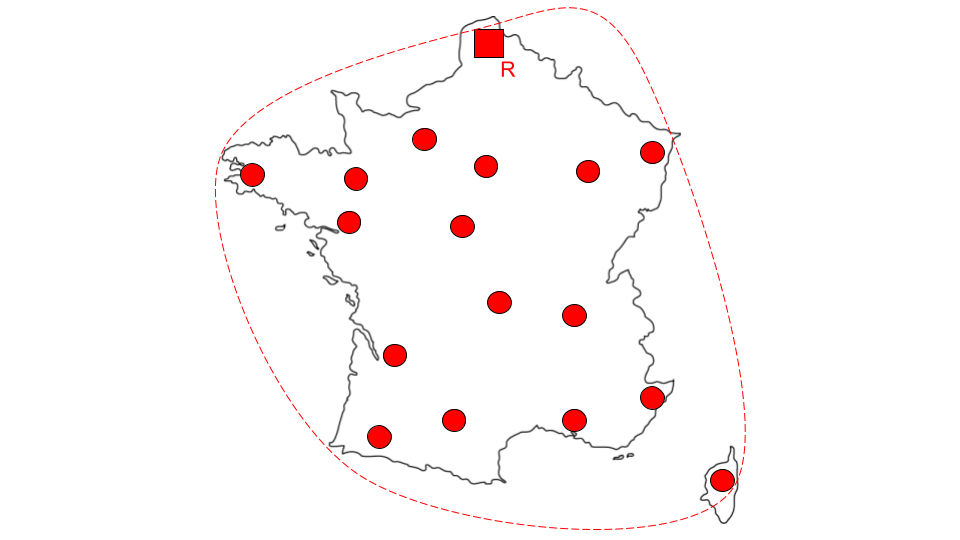
\includegraphics[trim=6cm 0.33cm 6cm 0.33cm, clip, width=0.24\textwidth]{img/Dynamic-partitioning-1.png}}
\hfill
\subfloat[\Process $G$ creates a second replica splitting the red set in two. \Processes request their closest replica host.\label{fig:partition_intuitionB}]{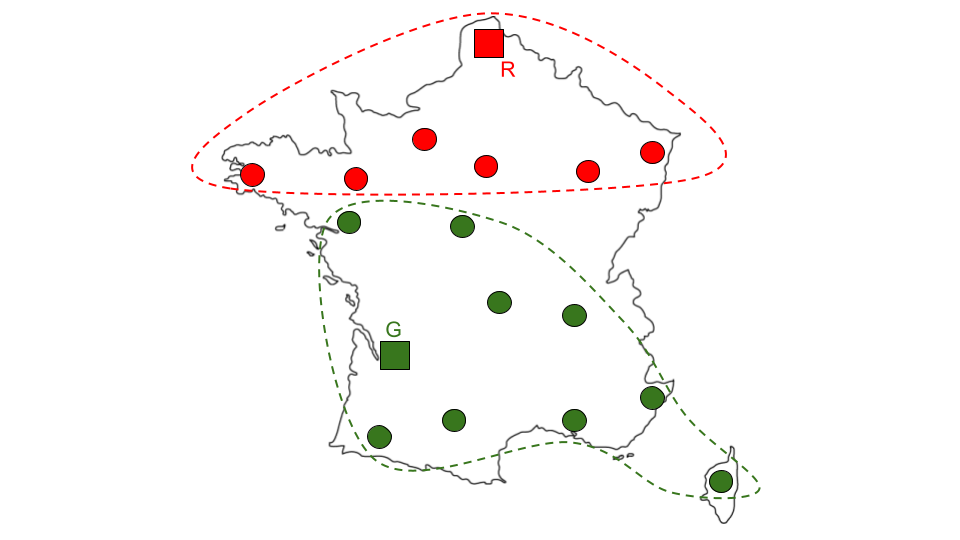
\includegraphics[trim=6cm 0.33cm 6cm 0.33cm, clip, width=0.24\textwidth]{img/Dynamic-partitioning-2.png}}\hfill
\subfloat[\Process $B$ creates another replica. \Process~$B$ needs to notify only a small subset of \processes.\label{fig:partition_intuitionC}]{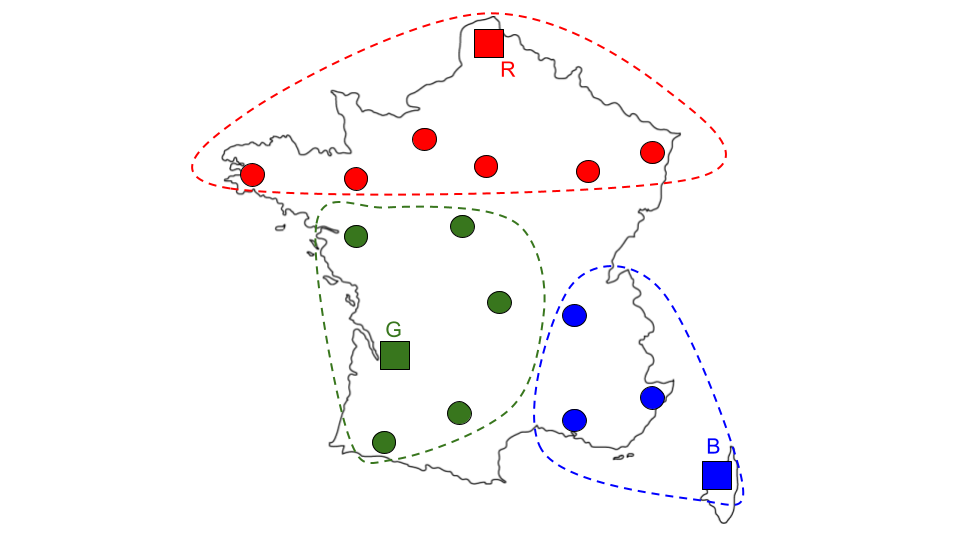
\includegraphics[trim=6cm 0.33cm 6cm 0.33cm, clip, width=0.24\textwidth]{img/Dynamic-partitioning-3.png}}\hfill
\subfloat[\Process $G$ destroys its replica. \Processes that belong to its partition must find the closest partition they are in.\label{fig:partition_intuitionD}]{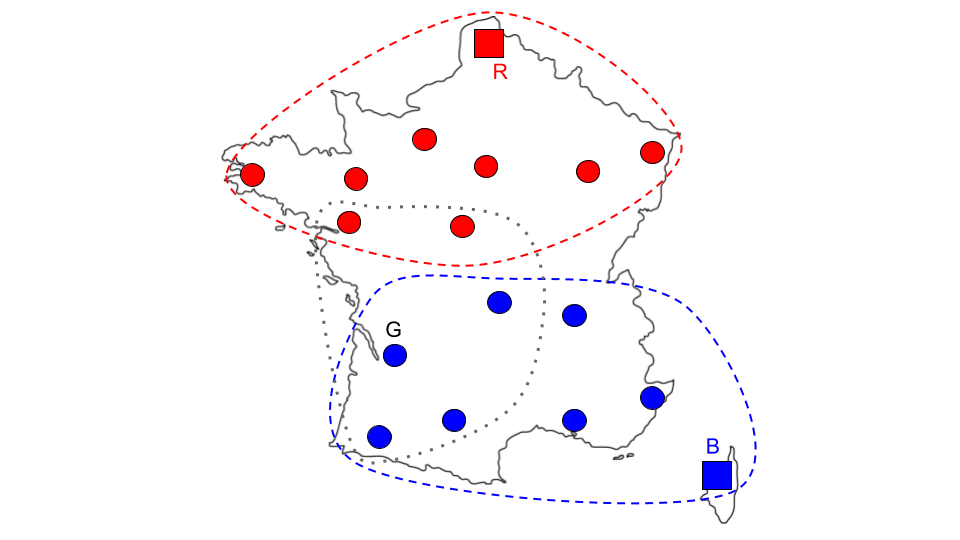
\includegraphics[trim=6cm 0.33cm 6cm 0.33cm, clip, width=0.24\textwidth]{img/Dynamic-partitioning-4.png}}
%
\caption{The french RENATER topology. Partitions
  grow and shrink depending on creations and removals of
  replicas.} \label{fig:partition_intuition}
\end{figure*}

%%% Local Variables: 
%%% mode: latex
%%% TeX-master: "../paper"
%%% ispell-local-dictionary: "english"
%%% End: 
 %% positioning

Such approaches are in contradiction with the objectives of Edge
infrastructures that aim at reducing the impact of latency as well as
the volume of data passing through the network.
%
First, accessing a remote \node to request content location(s) raises
hot spots and availability issues. But most importantly, it results in
additional delays~\cite{asrese2019measuring,doan2019tracing} that
occur even before the actual download started.
%
Second, the client gets a list of content locations at the discretion
of content indexing services. Without information about these
locations, it often ends up downloading from multiple replica hosts,
yet only keeping the fastest answer. In turn, clients either waste
network resources, or face slower response time.
%% there is no information to select the ``best'' node among the
%% possible candidates from which the content could be retrieved. In
%% most cases, this results in parallel requests performed by the
%% client node to each candidate with the goal of retrieving the
%% content as efficient as possible.

To address the aforementioned limitations, every \process that might
request or replicate content must also host its own content indexing
service in a fully decentralized fashion~\cite{kermarrec2015want}. At
any time, it can immediately locate the closest replica of specific
content.  A naive approach would be that every \process indexes and
ranks \emph{every live} replica along with its \emph{location}
information. When creating or destroying a replica, a \process would
notify all other \processes by broadcasting its
operation~\cite{birman1999bimodal,hadzilacos1994modular}. Unfortunately, this also contradicts Edge
infrastructure objectives, for such a protocol does not confine the
traffic generated to maintain its indexes. A \process may acknowledge
the existence of replicas at the other side of the network while there
already exists a replica next to it.

To mitigate the broadcasting overhead, a \process creating a replica
should notify all and only \processes that have no closer replica in
the system. This would create interconnected sets of \processes, or
\emph{partitions}, gathered around a \emph{source} being their
respective replica. A \process deleting its replica should notify all
members of its partition so they can rally their new
closest partition.
%
Some periodic advertisement
protocols~\cite{hemmati2015namebased,sohier2012physarum} already
provide both creation and deletion. Yet, their functioning
requires
\begin{inparaenum}[(i)]
\item to generate traffic even when the system is quiescent, and
\item the use of synchronous communications~\cite{sohier2012physarum}
  or physical-time-based intervals tuned according to network topology
  parameters such as network diameter~\cite{hemmati2015namebased}.
\end{inparaenum}

%% A ``simple'' way to tackle the aforementioned limitations would be to
%% maintain on each node composing the infrastructure and for each
%% content, an index of all replicas (and their ``distance'').  In such
%% an approach, each time a new replica is created or deleted, a message
%% is broadcasted from the node that performed the operation (\ie the
%% source) to all nodes, increasing the distance information at each hop.
%% %
%% In addition to being complicated for large-scale systems, maintaining
%% a global view on each node is useless as there is no interest to
%% inform a node of the creation/removal of a replica at the opposite of
%% the network (each node trying to get content from the ``closest''
%% one).  In other words, the broadcast should be limited to a partition
%% of the infrastructure, (\ie the subset of nodes that has to update the
%% current location for this particular content). Obviously, these
%% partitions depend and evolve according to concurrent operations made
%% by nodes (replica creation/removal) as well as dynamic changes in the
%% infrastructure (network failures, node apparitions/leaves).

\noindent In this paper, we address the content indexing challenge as
a distributed partitioning problem. Our contribution is threefold:

\begin{asparadesc} %% to remove left-margin :p
\item [$\bullet$] We highlight the properties that guarantee
  decentralized consistent partitioning in dynamic infrastructures. We
  demonstrate that concurrent creation and removal of partitions may
  impair the propagation of control information crucial for consistent
  partitioning. Yet, \processes are able to purge stale information
  forever using only neighbor-to-neighbor communication, hence leaving
  room for up-to-date information propagation, and eventually
  consistent partitioning.
  
\item [$\bullet$] We provide an implementation entitled \NAME that
  uses aforementioned principles to \underline{a}dapt its partitioning
  to creations and deletions of partitions even in dynamic systems
  where \nodes can join, leave, or crash at any time. \NAME's
  efficiency relies on a communication primitive called
  \underline{s}coped-broad\underline{cast}
   that enables epidemic
  dissemination of messages as long as receiving \processes verify an
  application-dependant predicate.
 
\item [$\bullet$] We evaluate \NAME through simulations using
  PeerSim~\cite{montresor2009peersim}. Results empirically show that
  \begin{inparaenum}[(i)]
  \item \NAME manages to quickly disseminate messages to the subset of
    relevant \processes;
  \item \NAME's overhead decreases when the number of partitions
    increases;
  \item \NAME does not generate traffic in quiescent systems; and
  \item \NAME enables consistent partitioning even in networks subject
    to physical partitioning.
  \end{inparaenum}
\end{asparadesc}

%% Ultimately, \NAME can constitute a novel building block for
%% geo-distributed services in need of efficient resource sharing in the
%% vicinity of regions. For instance, AS-cast could complement content
%% delivery infrastructures~\cite{triukose2011measuring} by efficiently
%% sharing between nodes attached to the same CDN server the locations of
%% web objects that have already been downloaded.  \NAME could even
%% constitute a decentralized implementation solving the multiple
%% destinations shortest path problem. 


%% Then, we propose \emph{\NAME}, a logical partitioning protocol that
%% uses \underline{s}coped broad\underline{cast} to \underline{a}dapt its
%% partitions, \ie scopes, to creations and deletions of partitions in
%% the system. Each source advertises its existence to all possibly
%% interested \processes, \ie only interconnected \processes of its
%% partition plus \processes bordering its partition. In turns, \NAME
%% scales well to the number of sources since the higher the number of
%% partitions, the earlier the dissemination stops.

%
%% In this paper, we propose a first implementation of such a protocol.
%% Entitled Adaptive Scoped broadcast (\NAME), 
%% our protocol relies on a primitive that forwards
%% messages until a certain condition is reached, \ie the scope. The
%% scope is defined by a boolean function (predicate) that returns
%% whether a message should be propagated or not around its
%% broadcaster. In the current scenario, the stop condition is related to
%% the distance to the nearest replica : if the message that a node receives
%% indicates a content has a longer distance than that which the node
%% knows then the transfer of the message is useless and so stopped.
%

% % %% \noindent In addition, \NAME guarantees that despite concurrent
% % %% operations, every \process eventually knows one, and only one, source:
% % %% its closest.
% % %% \NAME being reactive, when the system becomes quiescent, \processes do
% % %% not require further communications.

%% This primitive is used to guarantee that eventually, every node knows
%% its best partition, hence its closest replica, despite concurrent
%% events and receipt orders. Overall, \NAME is a wait-free reactive protocol for
%% dynamic logical partitioning.  Its overhead actually depends on
%% its operations and current partitions in the system. When the system
%% becomes quiescent, nodes eventually converge to their respective
%% partition and do not require further communication afterward.
% \TODO{talk about the proof}



%% We evaluated our protocol through two simulation scenarios using
%% \textit{Peersim}~\cite{montresor2009peersim}. First, we confirm that
%% \NAME allow consistent partitioning in an ad-hoc network composed of
%% 10K nodes.  Second, we illustrate how \NAME enables the lock down of
%% the traffic in dynamic inter autonomous systems.  More precisely, we
%% simulated a worldwilde infrastructure by duplicating the GEANT
%% topology - a real infrastructure spanning across Europe – and by
%% connecting these two clusters with a high latency link: 200 ms
%% simulating cross-continental communications such as Europe-America.

The rest of this paper is organized as
follows. Section~\ref{sec:background} illustrates the motivation and
problem behind our proposal.  Section~\ref{sec:adaptive} describes
dynamic consistent partitioning and its
implementation. Section~\ref{sec:experimentation} presents our
evaluations.  Section~\ref{sec:related_work} reviews related
work. Finally, Section~\ref{sec:conclusion} concludes and discusses
future work.
  

%%% Local Variables: 
%%% mode: latex
%%% TeX-master: "../paper"
%%% ispell-local-dictionary: "english"
%%% End: 
